% !TEX TS-program = xelatex
% !TEX encoding = UTF-8 Unicode
\documentclass[AutoFakeBold]{MyFormat}

\usepackage{listings}

\lstset{
 columns=fixed,       
 numbers=left,                                        % 在左侧显示行号
 numberstyle=\tiny\color{gray},                       % 设定行号格式
 frame=none,                                          % 不显示背景边框
 backgroundcolor=\color[RGB]{245,245,244},            % 设定背景颜色
 keywordstyle=\color[RGB]{40,40,255},                 % 设定关键字颜色
 numberstyle=\footnotesize\color{darkgray},           
 commentstyle=\it\color[RGB]{0,96,96},                % 设置代码注释的格式
 stringstyle=\rmfamily\slshape\color[RGB]{128,0,0},   % 设置字符串格式
 showstringspaces=false,                              % 不显示字符串中的空格
 language=c++,                                        % 设置语言
}

\begin{document}
%=====%
%
%封皮页填写内容
%
%=====%

% 标题样式 使用 \title{{}}; 使用时必须保证至少两个外侧括号
%  如: 短标题 \title{{第一行}},  
% 	      长标题 \title{{第一行}{第二行}}
%             超长标题\tiitle{{第一行}{...}{第N行}}

\title{{2022.05.24学习笔记}}
\author{Sillin Ini\\Pinyi Huang}
\maketitle
\thispagestyle{empty}
\newpage

%生成目录
\tableofcontents
\thispagestyle{empty}
\newpage

%文章主体
\mainmatter




% =======正文从第一章开始
\setcounter{chapter}{0}

\chapter{关于Transformer}

\par 原理图:

\begin{figure}[!h]
    \centering
    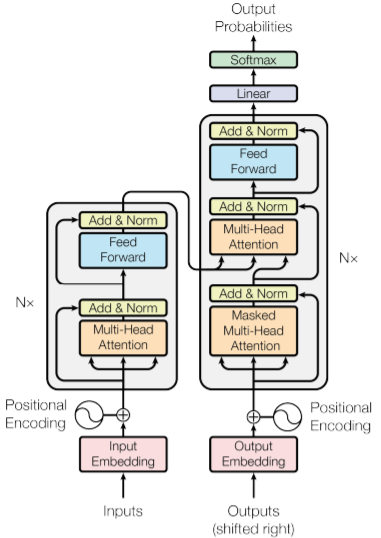
\includegraphics[width=0.4\linewidth]{figures/2022.05.24/pic1.png}
    \caption{Tranformer原理图(论文原图)}
\end{figure}

\section{Masked Self-Attention和Self-Attention的区别}
\par (1)self-attention的每个输出都考虑了所有输入

\begin{figure}[!h]
    \centering
    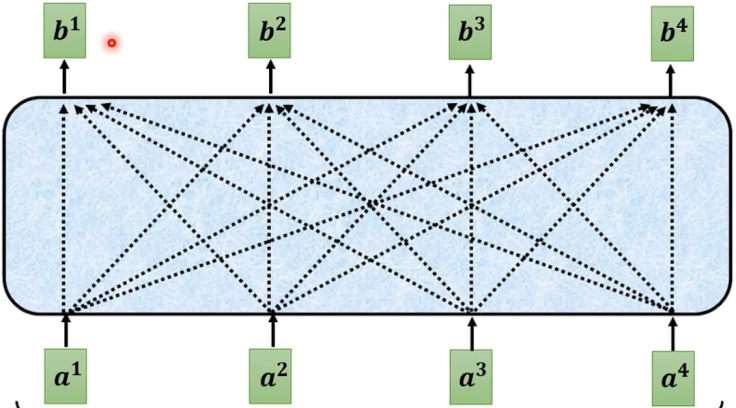
\includegraphics[width=0.6\linewidth]{figures/2022.05.24/pic2.png}
    \caption{self-attention并行工作原理图}
\end{figure}

\par 其具体的实现方法为:

\begin{figure}[!h]
    \centering
    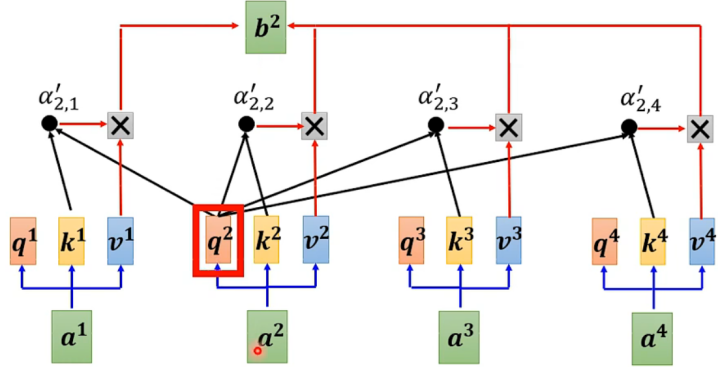
\includegraphics[width=0.6\linewidth]{figures/2022.05.24/pic3.png}
    \caption{self-attention具体得到各个输出的示意图}
\end{figure}

\par (2)masked之后,就只能考虑之前的输入(有点类似RNN,类似产生了时序关系)

\begin{figure}[!h]
    \centering
    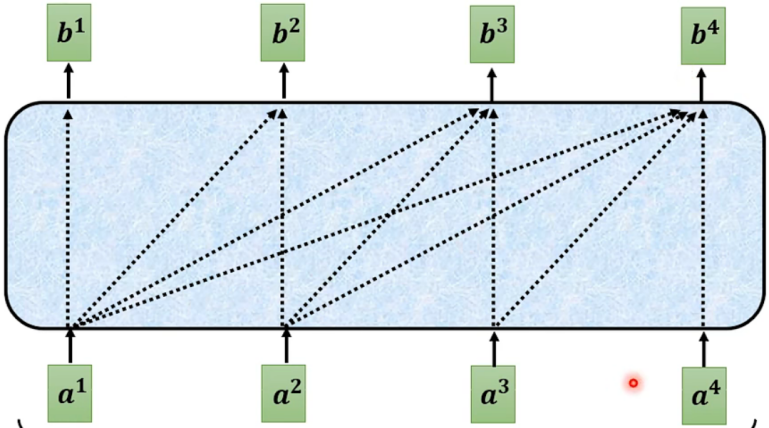
\includegraphics[width=0.6\linewidth]{figures/2022.05.24/pic4.png}
    \caption[]{masked self-attention原理图}
\end{figure}

\par mask之后的具体实现方法为:

\begin{figure}[!h]
    \centering
    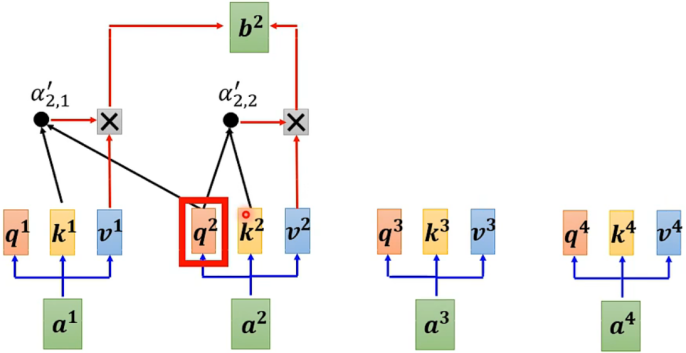
\includegraphics[width=0.6\linewidth]{figures/2022.05.24/pic5.png}
    \caption[]{masked self-attention具体得到各个输出的示意图}
\end{figure}

\par 其中,$b^2$的计算就只与$a^1$和$a^2$的$k^1$和$k^2$有关了,而非全部的key。

\section{为什么要使用Masked?}
\par 考虑到decoder的工作原理,其输入是一个一个输入、一个一个输出的,
当计算$b^2$的时候,$a^3$及之后的所有输入都还未到来,因此只能考虑之前的所有输入。
\par 这与Encoder当中的Self-Attention并行计算并不相同。


\chapter{Auto-Regressive自回归模型  VS  Non Auto-Regressive模型}
\section{两个模型的对比}

\begin{figure}[!h]
    \centering
    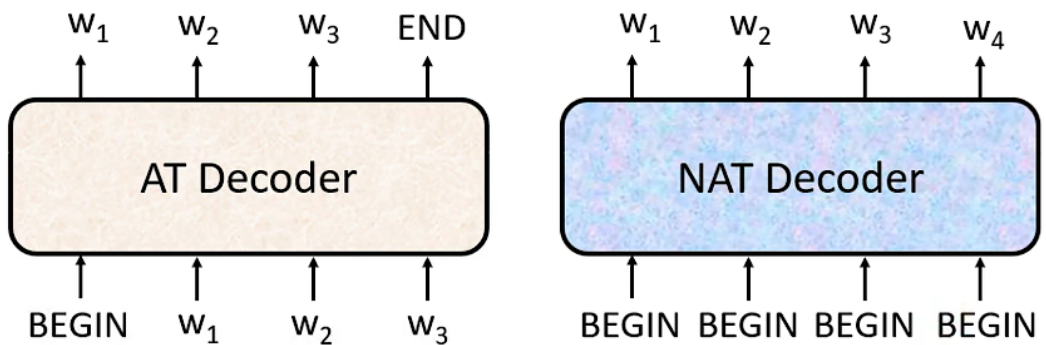
\includegraphics[width=0.6\linewidth]{figures/2022.05.24/pic6.png}
    \caption{AT模型和NAT模型的输入、输出对比}
\end{figure}

\begin{enumerate}
    \item 关于输入方式的不同: 
    \begin{itemize}
        \item AT模型一次给一个输入,并将该时刻输出作为下一时刻的输入,并以END结尾。
        \item NAT模型同时给一定数量的BEGIN向量,\textbf{\Large \underline{同时}}生成相同数量的输出,结束。
    \end{itemize}
    \item 怎样知道应该输出多少个字符?
    \begin{itemize}
        \item a.第一种方法是,再添加一个分类器classifier,
        输入一个要处理的对象,输出一个数字,
        该数字就是NAT Decoder同时输入的BEGIN的数量。
        \item b.第二种方法是,假设保证输出长度不超过300,就输入300个BEGIN。
        Decoder输出后,在其中第一个END处截断,只取前面的部分。
    \end{itemize}
    \item NAT模型的优势:
    \begin{itemize}
        \item 并行计算:同时输入一定数量的BEGIN,
        就能同时并行计算得到相应数量的输出;而AT模型中只能一个一个计算,速度更快。
        \item 它可以控制输出的长度
    \end{itemize}
    \item 但是,NAT模型的性能往往比AT模型的性能差。
\end{enumerate}

\section{Encoder - Decoder实现细节}

\begin{figure}[!h]
    \centering
    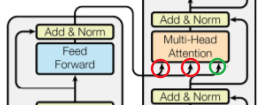
\includegraphics[width=0.5\linewidth]{figures/2022.05.24/pic7.png}
    \caption{Cross Attention部分的理解}
\end{figure}

\par Encoder和Decoder交互的部分叫做Cross Attention,
这也是Tranformer中最重要的部分。
\par 其中,左边的两个红箭头分别是来自Encoder的$Key$、$Value$($K$、$V$)矩阵,
绿箭头是来自Decoder的$Query$矩阵。
\par Attention的计算公式为:

\begin{equation}
    Attention(Q, K, V)=Softmax(\frac{QK^T}{\sqrt{d_k}})V
\end{equation}

\par 使用CrossEntropyLoss交叉熵训练,
使得总体的交叉熵值越小越好。这里的训练时,
可以使用一个Teacher Forcing(using the ground truth as input)
的情况进行训练,即使用正确的输出作为Decoder的每个输入。


\chapter{关于光流Optical Flow}

\section{关于光流:光流特点是运动信息}
\begin{enumerate}
    \item 光流在几个假设下起作用:
    \begin{itemize}
        \item 对象的像素强度在连续帧之间不会改变。
        \item 相邻像素具有相似的运动。
    \end{itemize}
    \item 稀疏光流:对某些像素点、角或者是边来说进行跟踪\\
    Lucas - Kanade光流方法:
    \begin{enumerate}
        \item 三个假设:
        \begin{itemize}
            \item 亮度恒定:像素点随时间变化时,
            其亮度值(像素灰度值)是恒定不变的。\\
            这是光流法的基本设定。(所有光流法都必须满足)
            \item 小运动:时间的变化不会引起位置的剧烈变化。\\
            这样才能利用相邻帧之间的位置变化引起的灰度值变化,
            去求取灰度对位置的偏导数。(所有光流法都必须满足)
            \item 空间一致:即前一帧中相邻像素点在后一帧中也是相邻的。\\
            \textbf{\Large \underline{这是LK光流法独有的假定}}。
            因为为了求取$x$, $y$方向的速度,
            需要建立多个方程联立求解。
            而空间一致假设就可以利用邻域n个像素点来建立n个方程。
        \end{itemize}
        \item 大致步骤:
        \begin{itemize}
            \item 首先进行角点检测cv2.goodFeaturesToTrack(),
            LK稀疏光流只能跟踪角点,将所有角点添加至一个列表中,
            以供后续进行跟踪
            \item 前一帧的角点和当前帧的图像作为输入来得到角点在当前帧的位置
            \item 当前帧跟踪到的角点及图像和前一帧的图像作为输入
            来找到前一帧的角点位置
            \item 得到角点回溯与前一帧实际角点的位置变化关系
            \item 以上一振角点为初始点,当前帧跟踪到的点为终点划线
        \end{itemize}
        \item LK金字塔:如当物体运动速度较快时,假设3不成立,
        那么后续的假设就会有较大的偏差,使得最终求出的光流值有较大的误差。
        因此需要使用LK金字塔进行求解。
    \end{enumerate}
    \item 稠密光流:\\
    基于前后两帧所有像素点的移动估算算法,其效果要比稀疏光流算法更好。
    由于要计算图像上所有点的光流,故计算耗时,速度慢。
    需要使用某种插值方法在比较容易跟踪的像素之间进行插值,
    以解决那些运动不明确的像素。\\
    与稀疏光流类似,稠密光流有两个\textbf{\Large \underline{目标}}:
    \begin{enumerate}
        \item 使得配准后的两张图像上每个对应点尽可能相同;
        \item 对于纯色区域的点,其光流计算式稍有不同,
        需要加入一个平滑项。平滑项的目的就是,
        对于特征比较弱的区域的点,其偏移量尽量向强特征点的偏移量靠近,
        或者说相邻两个特征点的偏移量相差不能太大,
        也就是偏移量的变化率不能太大。
    \end{enumerate}
    由此可得总体的目标函数如下:
    \begin{equation}
        \begin{split}
            \min_{u, v}E(u, v)=\int [\varphi (T(x, y)-I(x+u, y+u))+\\
            \lambda\cdot \psi(\left |\bigtriangledown u \right |, \left | 
            \bigtriangledown v \right |)]dxdy
        \end{split}
    \end{equation}
    前一部分是第一个目标的目标函数,后一部分是第二个目标的目标函数,
    其中$\lambda$是权重因子,$\varphi$和$\psi$被称为两个误差函数,
    其大致可以分为两大类:绝对值函数和二次函数,
    分别称为L1-光流(L1-范式)和L2-光流(L2-范式)。\\\\
    希望能减少图像中物体的运动速度。
    一个直观的方法就是,缩小图像的尺寸。
    假设当图像为400$\times$400时,物体速度为[16, 16],
    那么图像缩小为200$\times$200时,速度变为[8, 8]。
    缩小为100$\times$100时,速度减少到[4, 4]。\\
    所以在源图像缩放了很多以后,原算法又变得适用了。
    所以光流可以通过生成原图像的金字塔图像,逐层求解,
    不断精确来求得。简单来说上层金字塔(低分辨率)
    中的一个像素可以代表下层的两个。每一层的求解结果乘以2后加到下一层。
    \begin{figure}[!h]
        \centering
        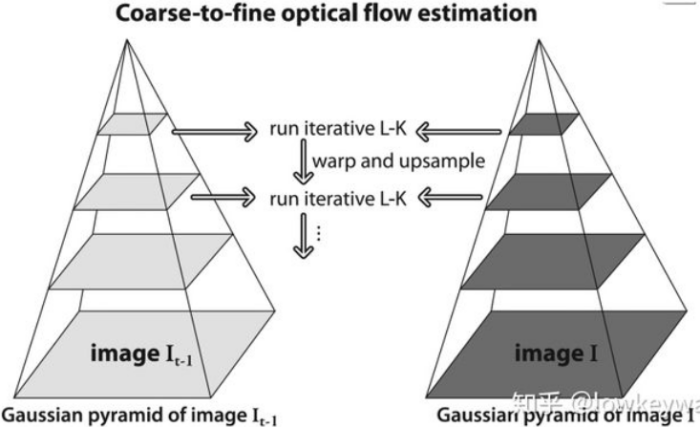
\includegraphics[width=0.6\linewidth]{figures/2022.05.24/pic8.png}
        \caption{LK金字塔示例}
    \end{figure}
    \\这就是calcOpticalFlowPyrLK中的maxLevel参数,
    图中有四层,则$maxLevel=3$,其中下层的宽度和高度均为上层的2倍。
\end{enumerate}


\section{LBP(\textit{Local Binary Pattern})局部二值模式}

\subsection{Basic LBP}
\par 不仅仅是“纹理特征”,因为可以把视频看作3D维度,即$x, y, t$三个维度,
因此可以在3D维度里提取LBP特征,即LBP也可以包含运动信息。
\par LBP特征中的像素值均为\textbf{\Large \underline{灰度值}},
因此需要先转为灰度图像。
\par 原始的LBP:
\begin{figure}[!h]
    \centering
    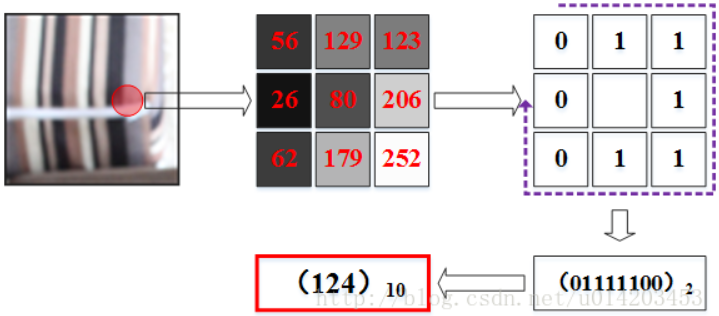
\includegraphics[width=0.6\linewidth]{figures/2022.05.24/pic9.png}
    \caption{LBP提取纹理特征过程示意图}
\end{figure}
\par 每一个图片可以划分为若干个Block,
每一个Block内划分为若干个Cell。
在Cell内部只用求一个LBP值,而非在图片上到处求。

\subsection{改进后的圆形LBP}
\par 使用符号为$LBP_{r, p}$其含义为半径为r,
总共等距取p个点。由于在圆弧上取点,因此坐标不可能全为整数,
非整数的点的灰度值一般采用\textbf{\Large \underline{双线性差值}}方法来确定。

\subsection{旋转不变性LBP}
\par 从LBP的定义可以看出,LBP算子是灰度不变的,但却不是旋转不变的,
图像的旋转就会得到不同的LBP值。
\par 不断旋转圆形邻域得到一系列初始定义的LBP值,取其最小值作为该邻域的LBP值。
\par 当一种编码在旋转过程中,能取到的所有值,在旋转不变LBP模式下,
都取同样的值,如$(0001)_2 = (0010)_2 = (0100)_2 = (1000)_2 = 1$
\par 如此一来,8位的LBP就可以被编码为
\textbf{\Large \underline{36}}种不同的取值。
\par 旋转LBP模式同样存在缺陷,
大量的实验证明LBP模式的36种情况在一幅图像中分布出现的频率差异较大,
得到的效果不是很好。因此人们提出了uniform LBP。

\subsection{Uniform LBP,LBP的等价模式}
\par 原始的LBP算子,随着邻域内采样点数的增加,二进制模式的种类是急剧增加的。
过多的二值模式对于特征的提取以及信息的存取都是不利的。
\par 将LBP算子用于人脸识别时,常采用的LBP模式的统计直方图来表达人脸信息,
而较多的模式种类将使得数据量过大,且直方图过于稀疏。因此,
需要对原始LBP模式进行降维,使得数据量减少的情况下能最好的代表图像的信息。

\subsection{LBP直方图}
\par 对于LBP直方图来说,横坐标是LBP编码值,纵坐标是占比:

\begin{figure}[!h]
    \centering
    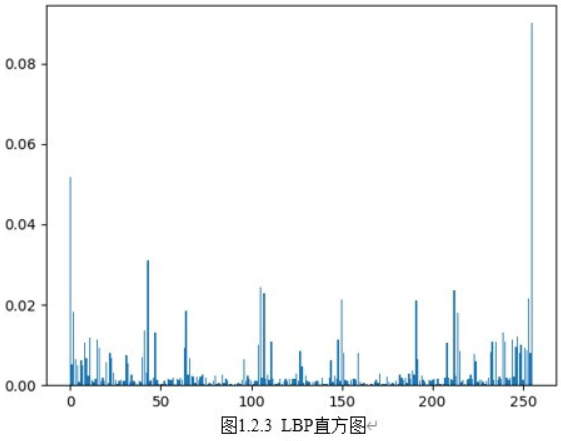
\includegraphics[width=0.4\linewidth]{figures/2022.05.24/pic10.png}
    \caption{LBP直方图}
\end{figure}

\par LBP可以得到图像的纹理部分:
\par 首先将图像转为灰度图像,之后求每个非边缘像素点的LBP值,
并将该像素点的值设为该值,遍历整个图像上的所有点,
最后就可以得到一个图像的纹理部分。

\section{VLBP(\textit{Volume LBP},体积局部二值模式)}
\par 对于$VLBP_{L,P,R}$来说,L表示时间间隔(如间隔L帧取样)、
P表示圆周上等距取P个点、R表示半径为R。
\par 对于时域来说,在$t_c-L$时刻、$t_c$时刻和$t_c+L$三个时刻进行取值。
其中$t_c$时刻的圆心表示了图像的整体亮度,对纹理分析没有帮助,则去掉。
因此一共有3P+2个点。
\par 大致实现方式如下,由外到内表示时间轴顺序:

\begin{figure}[!h]
    \centering
    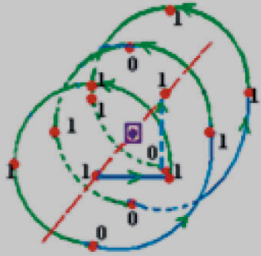
\includegraphics[width=0.4\linewidth]{figures/2022.05.24/pic11.png}
    \caption{VLBP取点顺序图}
\end{figure}

\par 按照顺序进行LBP编码,其权重依次从$2^0$到$2^{3P+1}$,
乘以0或1组成一个3P+2位的数。因此VLBP的直方图横坐标长度为$2^{3P+2}$。
\par 其中0和1是上图中的点依次和tc时刻圆心点的灰度值进行对比求得的。
\par 其融合了时间轴上的信息和LBP特征,因此能较好地提取动态纹理特征。
\par 其最重要的一点是,由3P+3个点的联合分布中提取出了3P+2个点的联合分布。
\par \textbf{\Large \underline{这一步产生了一定的信息损失,但由此实现了灰度不变性}}。
\par 这一步变换必须是各点相互独立才能实现,而这里进行了相互独立的假设,
实际情况可能不是如此,因此会产生一定的信息差
(\textit {However, we are willing to accept a possible small 
loss of information as it allows us to achieve invariance 
with respect to shifts in gray scale})。

\begin{figure}[!h]
    \begin{minipage}[t]{0.4\linewidth}
        \centering
        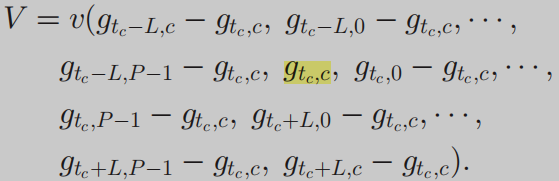
\includegraphics[width=\textwidth]{figures/2022.05.24/gongshi1.png}
        \centerline{(a) 各点的灰度值的联合分布原式}
    \end{minipage}%
    \hspace{0.1\linewidth}
    \begin{minipage}[t]{0.4\linewidth}
        \centering
        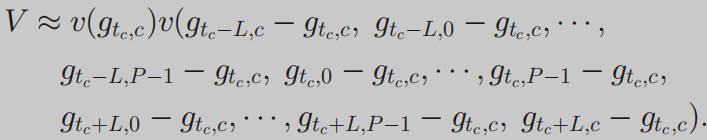
\includegraphics[width=\textwidth]{figures/2022.05.24/gongshi2.png}
        \centerline{(b) 进行各点无关假设,并提出后的联合分布式}
    \end{minipage}
    \caption{损失一定信息量实现灰度不变性的原理}
\end{figure}

\par 由此一来就得到了联合差分分布,就可以采用LBP方法提取纹理特征了。
\par 对于特征点数量P的选取:若P太大,则直方图将过长;若P太小,
则意味着会损失很多信息。由于数字的增长十分迅速,
这一点限制了VLBP的扩展和适用性。
\par 同时,当L大于1时,相邻帧的信息就会被忽略了。

\section{双线性差值的OpenCV计算公式}

\begin{figure}[!h]
    \centering
    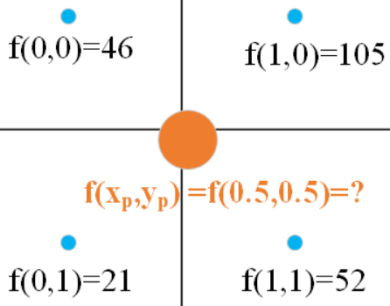
\includegraphics[width=0.6\linewidth]{figures/2022.05.24/pic12.png}
    \caption{双线性差值计算公式}
\end{figure}

\par 在图中,已知各点的像素值,求$x, y\in (0, 1)$的双线性差值。
\par 其计算公式为:

\begin{equation}
    f(P)=f(x, y)\approx 
    \begin{bmatrix}
        1-x & x
    \end{bmatrix}
    \begin{bmatrix}
        f(0, 0) & f(0, 1)\\
        f(1, 0) & f(1, 1)
    \end{bmatrix}
    \begin{bmatrix} 
        1-y\\y
    \end{bmatrix}
\end{equation}

\par 或者可以写成:
\begin{equation}
    f(P)=f(x, y) \approx (1-x)(1-y)f(0, 0)+x(1-y)f(1, 0)+(1-x)yf(0, 1)+
    xyf(1, 1)
\end{equation}

\section{LBP-TOP(\textit{LBP from Three orthogonal planes})}
\par 普通的LBP只考虑了XY轴,因此只能用于单张图片进行纹理特征提取。
\par 在LBP-TOP中额外考虑了一个随时间变化的t轴,
由此可以适用于视频片段的纹理特征提取。
LBP-TOP分别考虑了X-Y、X-T和Y-T轴,在三个面上分别进行LBP特征提取,
将三个面的直方图直接连接起来,就得到了LBP-TOP的直方图。
\par LBP-TOP的直方图横坐标bin长度为$2^P\times 3$,
其中2P是指其编码一共有这么多种可能,3是指三个正交平面直接相连。
\\\hspace*{\fill}
\par 对于LBP-TOP来说,T轴上的半径和XY上的半径不宜相同。
尤其对于高分辨率、低帧率的图像来说,在T轴上相同的时间间隔内,
纹理可能发生剧烈变化。因此整体看来,LBP-TOP的取样是一个椭球。\\
\hspace*{\fill}

\par LBP-TOP接收六个参数,如:$LBP-TOP_{P_{XY}, P_{XT},
P_{YT}, R_X, R_Y, R_T}(x_{c, t}, y_{c, t})$
\\\hspace*{\fill}

\par LBP-TOP对于面部表情识别来说,
最佳的半径选择(x, y, t)是$\{1, 1, 2\}$,
而在\textbf{\Large \underline{微表情}}识别来说是$\{1, 1, 4\}$。

\section{LBP-SIP(\textit{LBP with Six Intersection Points},
具有六个相交点的LBP)}

\par 注意,在LBP-TOP的计算中,每个邻居像素被使用多次,
并且在相交平面集合中只有6个不同的邻居点。

\par LBP-SIP认为相交的六个点就已经带来了足够描述时空动态纹理的足够信息,
因此只需要对这六个点进行特征提取并进行分类就已经足够了。

\par LBP-SIP接收四个参数,如:

\par LBP-SIP性能优于LBP-TOP,原因是高纬度的特征通常会受到维度诅咒,
即所表示的数据变得越来越稀疏,影响了分类能力。这一点LBP-SIP做得更好,
其缩减了特征的维数,使得数据更紧凑、计算复杂度更低。


\chapter{使用神经网络进行微表情识别}

\section{双时间尺度卷积神经网络(\textit{Dual Time Scaled CNN, DTSCNN})}

\par 对于传统意义上的CNN来说,训练一个神经网络需要一个比较大的数据集。
而微表情识别这一方面并没有这么大的数据集,因此无法使用传统的CNN进行识别。
\par 在现存的微表情数据集上进行训练CNN,所产生的后果是会带来及其严重的过拟合,
这对于微表情识别来说是不能接受的。
\par 而DTSCNN则尝试了从三个不同的层面来防止类似问题的发生:
\begin{enumerate}
    \item 使用两个浅层的神经网络进行特征提取
    \item 使用数据增强和更高的Dropout比率
    \item 使用了CASME I和CASME II来训练神经网络
\end{enumerate}
\hspace*{\fill}
\par 为了使神经网络能够获取更高级别的特征,使用神经网络训练的特征是光流,
而不是原始数据。
\par 同时,为了解决已存在的微表情数据集过小的问题,DTSCNN设计了独特的
数据增强方法,以获得相对来说足够大的训练集:
\begin{figure}[!h]
    \centering
    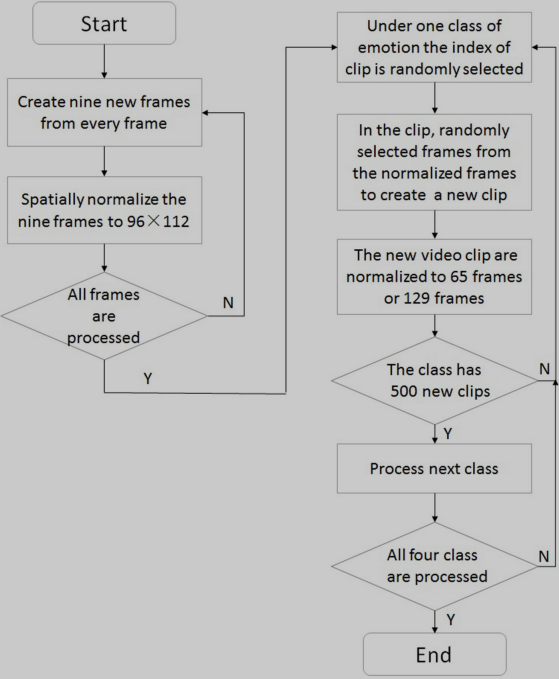
\includegraphics[width=0.4\linewidth]{figures/2022.05.24/DTSCNN.png}
    \caption{DTSCNN流程图}
\end{figure}
\par 同时还将最后FC层的Dropout比例设置为了0.5,
这也在一定程度上缓解了过拟合问题。

\section{基于面部图表示学习和面部动作单元融合的微表情识别
\textit{FGRMER}}
\par FGRMER其全称为:\textit{Micro-Expression Recognition Based on Facial
Graph Representation Learning and Facial Actcion Unit Fusion}
\subsection{FGRMER的步骤大致为}
\begin{enumerate}
    \item 使用DConv将各个patches视为许多个通道,学习其中的特征,即点学习。
    \item 使用Encoder of Transformer来学习点之间的关系,即边学习。
    由此就学习到了一个面部图表示。
    \item 使用AU-GCN,通过嵌入和GCN学习动作单元矩阵。
    \item 设计了一个将动作单元矩阵与面部图表示进行结合的融合模型。
\end{enumerate}

\subsection{FGRMER相对于其他方法的优势}
\par 肌肉移动映射在微表情领域上时,其变化主要是几何变化。相对来说,
纹理的变化是非常微弱的,并且容易收到各种其他因素的干扰。
\par 由此来说,基于面部纹理特征的\textbf{\Large \underline{LBP}}
方法不会是微表情方面最好的方法。
\\\hspace*{\fill}
\par \textbf{\Large \underline{MagNet}}通过转移学习(Transfer Learning)
将深度学习引入了微表情增强方面,产生了当时最好的效果。
这证明了增强后的几何特征对微表情识别有着十分重要的贡献。
\par 但是MagNet随后的操作中,其将二维特征粗鲁的直接降成了一维,
这造成了空间信息的损失;同时这个方法也没有考虑到Action Unit(AU)的机制。
因此这个方法同样具有提升的空间。
\\\hspace*{\fill}

\par 关于AU特征矩阵的获取,
使用到了\textbf{\Large \underline{MER-GCN}}模型[20]。




\chapter{杂七杂八的知识}

\section{图像金字塔}
\par 图像金字塔实际上是一张图片在不同尺度下的集合,
即原图的上采样和下采样集合。金字塔的底部是高分辨率图像,
而顶部是低分辨率图像。我们将一层一层的图像比喻成金字塔,
层级越高,则图像越小,分辨率越低。
\begin{figure}[!h]
    \centering
    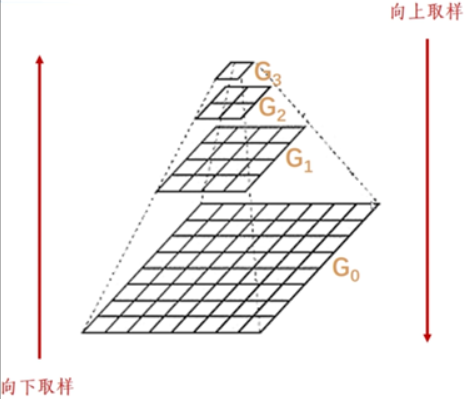
\includegraphics[width=0.4\linewidth]{figures/2022.05.24/pic16.png}
    \caption{金字塔示例图}
\end{figure}

\begin{enumerate}
    \item 高斯金字塔$G_i$:\\
    采用高斯滤波的方法形成的金字塔。\\
    上采样:将行列扩充为原来的2倍,偶数行列置0,然后采用高斯滤波。\\
    下采样:先用高斯滤波(高斯核要和上面相同),再去掉偶数行列。
    \item 拉普拉斯金字塔:
    \begin{equation}
        L_i=G_i-PyrUp(PyrDown(G_i))
    \end{equation}
    即拉普拉斯金字塔的每一层是根据高斯金字塔计算得来的,
    高斯金字塔的每一层减去其先下采样再上采样后的值。\\
    拉普拉斯金字塔保留的是残差,为图像还原做准备。
\end{enumerate}

\section{关于矩阵求导}

\subsection{对于标量函数和向量函数}
\par 标量函数:输出为标量(一个数)的函数,输入可以为一个向量。
\par 向量函数:输出为向量(或矩阵甚至是张量)的函数,如
\begin{equation}
    f(x)=
    \begin{bmatrix}
        f_1(x)=x\\f_2(x)=x^2
    \end{bmatrix}, R \to R^2
\end{equation}

\par 输入:可以是标量、向量、矩阵
\par 输出:可以是标量、向量、矩阵

\subsection{矩阵求导的\textbf{\Large \underline{本质}}}

\par $\frac{dA}{dB}$:矩阵A中的每个元素对矩阵B中的每个元素求导
\par 若$A_{p\times q}$和$B_{m\times n}$,
则$(\frac{dA}{dB})_{p\times q\times m\times n}$

\subsection{求导方法}
\par 标量不变,向量拉伸;前面$f(x)$横向拉,后面$x$纵向拉
例子:
\begin{enumerate}
    \item $R^n \to R$,即$x = (x_1, ..., x_n)$,$f(x)=f(x_1, ..., x_n)$
    \begin{figure}[!h]
        \centering
        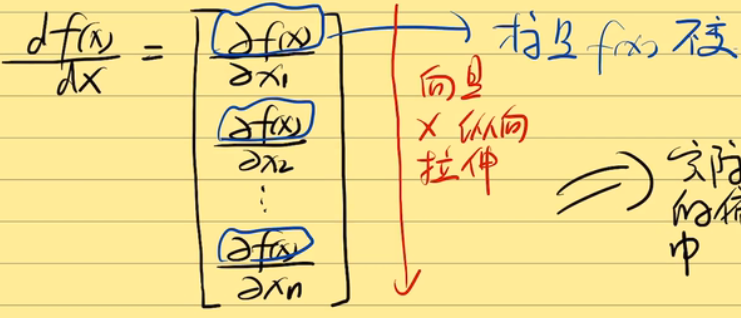
\includegraphics[width=0.4\linewidth]{figures/2022.05.24/pic13.png}
    \end{figure}
    \item $R \to R^n$,即$f(x)=[f_1(x), ..., f_n(x)]^T$
    \begin{figure}[!h]
        \centering
        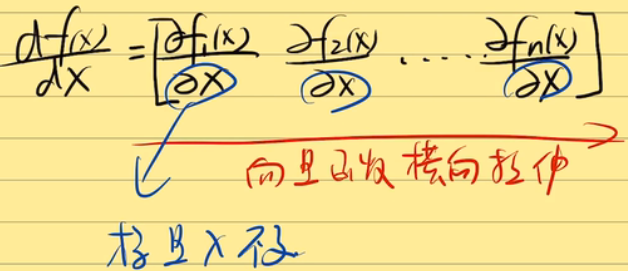
\includegraphics[width=0.4\linewidth]{figures/2022.05.24/pic14.png}
    \end{figure}
    \item $R^m \to R^n$,即以上两种组合:
    \begin{figure}[!h]
        \centering
        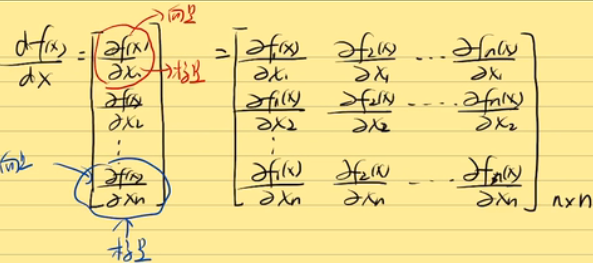
\includegraphics[width=0.4\linewidth]{figures/2022.05.24/pic15.png}
    \end{figure}
\end{enumerate}

\subsection{二次型求导公式}
\begin{equation}
    \frac{dx^TAx}{dx}=(A+A^T)x
\end{equation}


% \setcounter{chapter}{0}
\chapter{关于相关代码}

\section{cv2.goodFeaturesToTrack()}

\par 该函数查找图像或指定图像区域中最突出的角点。
\par corners = cv.goodFeaturesToTrack(image, maxCorners, 
qualityLevel, minDistance[,\\ corners[, mask[,
blockSize[, useHarrisDetector[, k]]]]])
\par 输入的参数分别是:
\begin{itemize}
    \item image: 输入图像,是八位的或者32位浮点型,
    单通道图像,所以有时候用灰度图
    \item maxCorners: 返回最大的角点数,是最有可能的角点数,
    如果这个参数不大于0,那么表示没有角点数的限制。
    \item qualityLevel: 图像角点的最小可接受参数,
    质量测量值乘以这个参数就是最小特征值,小于这个数的会被抛弃。
    \item minDistance: 返回的角点之间最小的欧式距离。
    \item mask: 检测区域。如果图像不是空的
    (它需要具有CV\_8UC1类型和与图像相同的大小),它指定检测角的区域。
    \item blockSize: 用于计算每个像素邻域上的导数协变矩阵的平均块的大小。
    \item useHarrisDetector:选择是否采用Harris角点检测,默认是false。
    \item k:Harris检测的自由参数
\end{itemize}


\section{cv2.calcOpticalFlowPyrLK()}
\par 迭代计算LK稀疏光流函数
\par lk\_params = dict(winSize=(15, 15),
maxLevel=2,
criteria=(cv2.TERM\_CRITERIA\_EPS | cv2.TERM\_CRITERIA\_COUNT, 10, 0.03))
\par p1, st, err = cv2.calcOpticalFlowPyrLK(img0, img1, p0, None,
**lk\_params)
\begin{itemize}
    \item p1表示光流检测后的角点位置;
    \item st表示是否是运动的角点;
    \item err表示是否出错;
    \item img0表示输入前一帧图片;
    \item img1表示后一帧图片;
    \item p0表示需要检测的角点;
    \item lk\_params:
    \begin{itemize}
        \item winSize表示选择多少个点进行$u$和$v$的求解;
        \item maxLevel表示空间金字塔的层数;
    \end{itemize}
\end{itemize}


\end{document}